\subsection{Differentiable Parametric Fur Representation}
\label{sec:parametric-fur}

We represent animal fur as explicit, surface-rooted strands with interpretable
grooming controls. In contrast to an unconstrained set of independent Gaussian
primitives, every strand retains a semantic mesh root, a continuous centerline,
and root-to-tip geometry and appearance profiles. The representation is
differentiable up to the discrete choice of its Gaussian segment count.

\paragraph{Surface-rooted 3D flow.}
For a root $\mathbf{x}_r$ on the body mesh, we construct the orthonormal frame
$\mathbf{F}_r=[\mathbf{t}_r,\mathbf{b}_r,\mathbf{n}_r]$ from the surface
tangent, bitangent, and outward normal. A normalized local groom direction
$\mathbf{d}^{\mathrm{loc}}_r$ is mapped to world space as
\begin{equation}
    \mathbf{d}_r =
    \frac{\mathbf{F}_r\mathbf{d}^{\mathrm{loc}}_r}
         {\lVert\mathbf{F}_r\mathbf{d}^{\mathrm{loc}}_r\rVert_2}.
\end{equation}
This defines a genuine 3D direction field rather than an image-plane flow,
which is essential around limbs, the belly, and the tail.

\paragraph{Normal-to-flow brush backbone.}
Given positive endpoint length $L_r$, the nominal strand tip is
$\mathbf{x}^{\mathrm{tip}}_r=\mathbf{x}_r+L_r\mathbf{d}_r$.
We model the smooth turn from the skin normal toward the groom direction using
a quadratic Bezier backbone
\begin{equation}
    \mathbf{B}_r(u)=(1-u)^2\mathbf{x}_r
    +2(1-u)u\mathbf{c}_r+u^2\mathbf{x}^{\mathrm{tip}}_r,
    \qquad u\in[0,1].
\end{equation}
Let
\begin{align}
    \mathbf{c}^{\mathrm{straight}}_r
        &=\tfrac{1}{2}(\mathbf{x}_r+\mathbf{x}^{\mathrm{tip}}_r),\\
    \mathbf{c}^{\mathrm{corner}}_r
        &=\mathbf{x}_r+
        \langle L_r\mathbf{d}_r,\mathbf{n}_r\rangle\mathbf{n}_r.
\end{align}
The control point is
\begin{equation}
    \mathbf{c}_r=\mathbf{c}^{\mathrm{straight}}_r+
    s_r\left\lVert
        \mathbf{d}_r-\langle\mathbf{d}_r,\mathbf{n}_r\rangle\mathbf{n}_r
    \right\rVert_2
    (\mathbf{c}^{\mathrm{corner}}_r-\mathbf{c}^{\mathrm{straight}}_r),
\end{equation}
where $s_r\in[0,1]$ is brush stiffness. The tangential-difference factor
continuously suppresses curvature when the groom direction is already close to
the normal. Thus $s_r=0$ yields a straight strand, while increasing $s_r$
produces one smooth normal-to-flow turn without a threshold or a second bend
field.

\paragraph{Independent curl and micro-frizz.}
Let $\boldsymbol{\tau}_r(u)$ be the backbone tangent and
$\mathbf{s}_r(u),\mathbf{o}_r(u)$ be transported transverse axes. With the
root-preserving envelope $E(u)=u^2(3-2u)$, curl is
\begin{equation}
\begin{split}
    \mathbf{C}_r(u)=r_rE(u)\big[&
    (\sin\theta_r(u)-\sin\phi_r)\mathbf{s}_r(u)\\
    &+(\cos\theta_r(u)-\cos\phi_r)\mathbf{o}_r(u)\big],
\end{split}
\end{equation}
where $\theta_r(u)=\phi_r+2\pi f_ru$, $f_r$ is turns per strand, and $\phi_r$
is phase. We optimize the dimensionless curl ratio $\rho_r$ and decode
$r_r=L_r\rho_r$, so one control has comparable geometry across short and long
fur. Band-limited geometric
micro-frizz is
\begin{equation}
    \mathbf{R}_r(u)=a_rE(u)
    \left[\eta^s_r(u)\mathbf{s}_r(u)+\eta^o_r(u)\mathbf{o}_r(u)\right],
\end{equation}
where the optimized dimensionless amplitude $\alpha_r$ is decoded as
$a_r=L_r\alpha_r$, and $\eta^s_r,\eta^o_r$ are deterministic smooth noise
signals generated from a persistent per-strand seed. Both details are
evaluated around the same undeformed backbone,
\begin{equation}
    \mathbf{P}_r(u)=\mathbf{B}_r(u)+\mathbf{C}_r(u)+\mathbf{R}_r(u),
\end{equation}
making them additive and independently editable. Here micro-frizz describes
geometric roughness and is distinct from material BRDF roughness.

\paragraph{Root-to-tip profiles.}
Each strand stores root and tip widths $(w^0_r,w^1_r)$ and taper exponent
$\gamma_r>0$,
\begin{equation}
    w_r(u)=w^0_r(1-u^{\gamma_r})+w^1_ru^{\gamma_r}.
\end{equation}
Color and opacity are continuous root-to-tip profiles,
\begin{equation}
    \mathbf{a}_r(u)=(1-u)\mathbf{a}^0_r+u\mathbf{a}^1_r,
    \qquad
    \alpha_r(u)=(1-u)\alpha^0_r+u\alpha^1_r.
\end{equation}

\paragraph{Strand-to-Gaussian conversion.}
We adaptively resample each curve according to physical length and geometric
complexity. Adjacent samples $\mathbf{p}_{r,j}$ and
$\mathbf{p}_{r,j+1}$ define one anisotropic Gaussian with
\begin{equation}
    \boldsymbol{\mu}_{r,j}=\tfrac{1}{2}
    (\mathbf{p}_{r,j}+\mathbf{p}_{r,j+1}),
    \qquad
    \mathbf{s}_{r,j}=\left(
    \tfrac{\kappa}{2}\lVert\Delta\mathbf{p}_{r,j}\rVert_2,
    \bar{w}_{r,j},\bar{w}_{r,j}\right),
\end{equation}
whose principal axis follows $\Delta\mathbf{p}_{r,j}$. Longer or more curved
strands automatically receive more contiguous Gaussian segments. The discrete
segment count is detached, while positions, orientations, scales, colors, and
opacities remain differentiable functions of the continuous groom parameters.

\begin{figure*}[t]
    \centering
    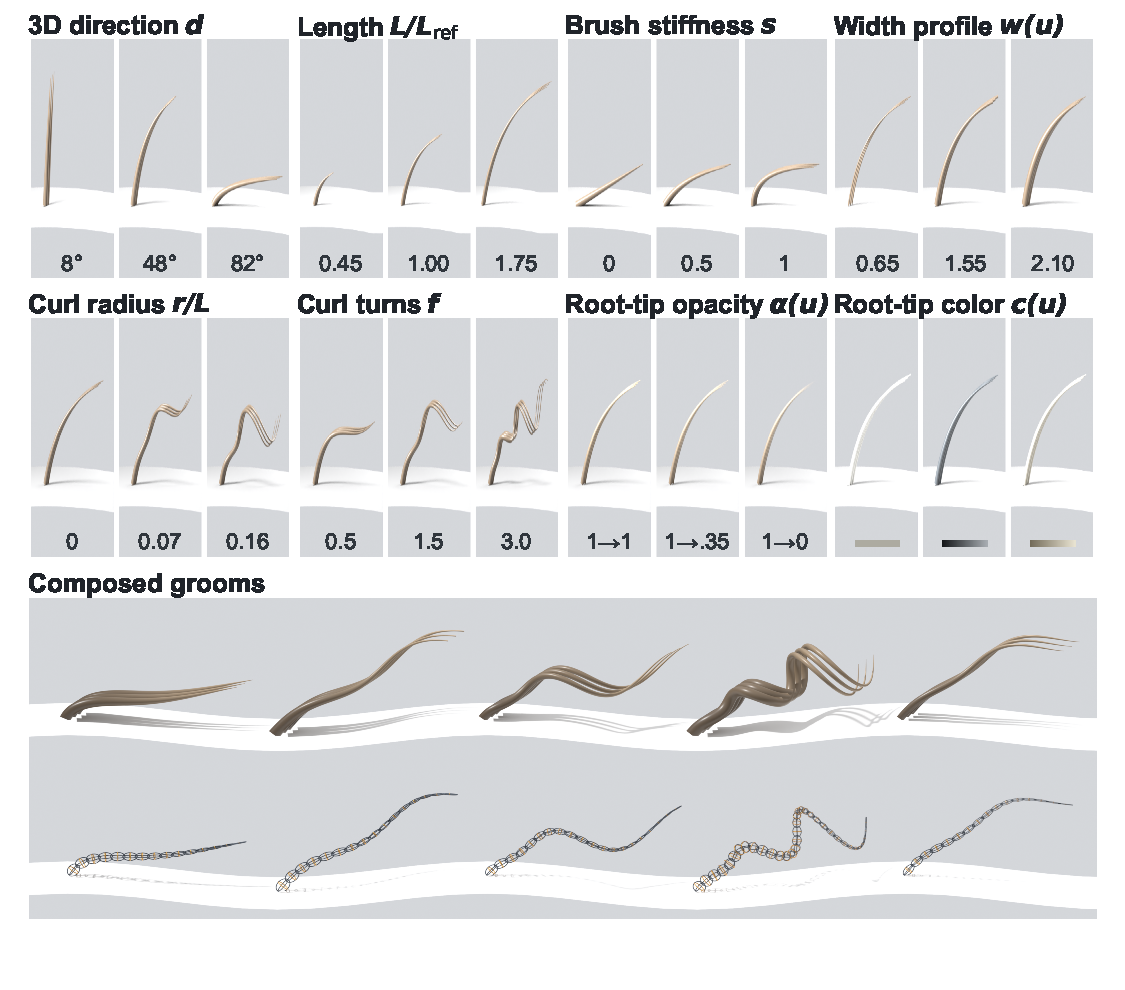
\includegraphics[width=\textwidth]
    {method/fig_parametric_groom_controls.pdf}
    \caption{\textbf{Interpretable differentiable groom controls.}
    Single-variable sweeps show the effects of 3D direction, length, brush
    stiffness, width profile, curl radius, curl turns, geometric micro-frizz,
    and root-to-tip color. The displayed geometric sweeps use
    $\hat{L}=L/L_{\mathrm{ref}}$, $\hat{r}=r/L$, and
    $\hat{a}=a/L$. Each strand is rendered over a shallow convex
    receiver to expose its three-dimensional shape and contact shadow. The
    composed examples combine multiple controls; the aligned lower row shows
    the corresponding adaptive anisotropic Gaussian initialization after all
    geometric deformation.}
    \label{fig:parametric-groom-controls}
\end{figure*}
